% VUT FIT MITAI
% MSZ 2021/2022
% Author: Vladimir Dusek
% Login: xdusek27

%%%%%%%%%%%%%%%%%%%%%%%%%%%%%%%%%%%%%%%%%%%%%%%%%%%%%%%%%%%%%%%%%%%%%%%%%%%%%%%%

\chapter{Symetrická kryptografie. Vlastnosti, vlastnosti bezpečného algoritmu, délka klíče, útok silou,
příklady symetrických algoritmů, Feistelovy šifry, DES, režimy činnosti, proudové šifry.}

%%%%%%%%%%%%%%%%%%%%%%%%%%%%%%%%%%%%%%%%%%%%%%%%%%%%%%%%%%%%%%%%%%%%%%%%%%%%%%%%

\section{Metadata}

\begin{itemize}
    \item Předmět: Kryptografie (KRY)
    \item Přednáška:
    \begin{itemize}
        \item 3) Symetrická kryptografie. Vlastnosti, vlastnosti bezpečného algoritmu, délka klíče, útok silou.
        \item 4) Příklady symetrických algoritmů, Feistelovy šifry, DES, struktura, činnost, slabiny, režimy činnosti.
        \item 5) Typické aplikace symetrické kryptografie.
    \end{itemize}
    \item Záznam:
    \begin{itemize}
        \item 2021-02-22
    \end{itemize}
\end{itemize}

%%%%%%%%%%%%%%%%%%%%%%%%%%%%%%%%%%%%%%%%%%%%%%%%%%%%%%%%%%%%%%%%%%%%%%%%%%%%%%%%

\section{Úvod a kontext}

\paragraph*{Symetrická kryptografie} Algoritmy používají k šifrování i dešifrování stejný klíč. Výhodou symetrických šifer je jejich nízká výpočetní náročnost. Asymetrické šifry mohou být i stotisíckrát pomalejší. Nevýhodou je nutnost sdílení tajného klíče, takže jedna strana musí klíč vygenerovat a potom ho bezpečným způsobem předat druhé straně.

\paragraph*{Typy útoků} \begin{itemize}
    \item Ciphertext Only Attack (COA) -- Útočník zná pouze zašifrovaný text a snaží se zjistit klíč nebo otevřený text. Nejčastěší případ.
    \item Known Plaintext Attack (KPA) -- Útočník zná zašifrovaný text a otevřený text a snaží se zjistit klíč.
    \item Chosen Plaintext Attack (CPA) -- Útočník zná to co v KPA a navíc si text může zvolit.
    \item Brute force -- Útok silou, zkouší se všechny možné klíče, dokud se nenajde ten správný.
\end{itemize}

\begin{figure}[H]
    \centering
    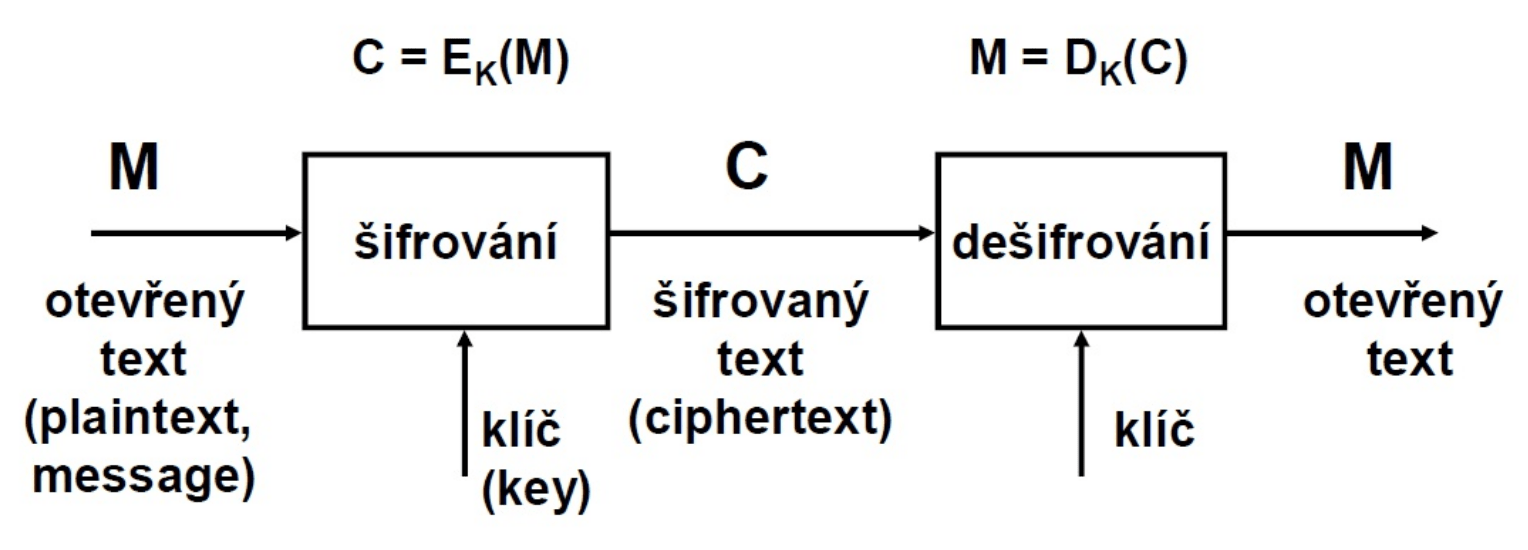
\includegraphics[width=0.75\linewidth]{50/kryptografie.png}
    \caption{Princip kryptografie, podle klíčů dělíme na symetrickou (tajný klíč) a asymetrickou (veřejný klíč, soukromý klíč).}
\end{figure}

\paragraph*{Bezpečný algoritmus} V moderní kryptografii je nepřijatelné utajování algoritmů (\textit{security by obscurity}). Jediné co je tajné je klíč (\textit{security by design}). Symetrický algoritmus je považován za bezpečný, pokud neexistuje rychlejší útok než útok silou.

\paragraph*{Délka klíče} Dnes je považováno 80 bitů a více za dostatečné. Typicky se délka zaokrouhluje na mocninu 2. Klíče symetrických algoritmů jsou kratší než asymetrických. Konkrétně: DES -- 56b, 3DES -- 112, AES -- variabilní.

\paragraph*{Využití} Symetrická kryptografie je vhodná pro šifrování většího objemu dat. Narozdíl od asymetrické, která je pro tento účel příliš pomalá. Proto např. HTTPS využívá asymetrickou kryptografii pro výměnu symetrických klíčů a poté symetrickou kryptografii pro šifrování provozu.

\paragraph*{Vlastnosti moderní kryptografie} \begin{itemize}
    \item Důvernost -- Utajení informace. Bez znalosti klíče, není možné data číst.

    \item Autentizace -- Prokázání, že zprávu skutečně poslal odesílatel a nikoliv útočník, který se za odesílatele vydává.

    \item Integrita -- Prokázání, že nikdo nemohl data po cestě od odesílatele k příjemci změnit. Ochrana proti neoprávněné, neodhalené modifikaci zprávy.

    \item Nepopiratelnost -- Pokud odesílatel data poslal, nemůže tuto skutečnost popřít.
\end{itemize}

%%%%%%%%%%%%%%%%%%%%%%%%%%%%%%%%%%%%%%%%%%%%%%%%%%%%%%%%%%%%%%%%%%%%%%%%%%%%%%%%

\section{Blokové šifry}

Blokové šifry šifrují data po blocích pevně stanovené délky (64b, 128b, 256b, \dots). Pokud je dat více, rozdělí se na více bloků, přičemž do zbylého místa v posledním je umístěn \textit{padding}. Příklady blokových šifer: \begin{itemize}
    \item Feistelova šifra
    \item Data Encryption Standard (DES)
    \item Triple Data Encryption Algorithm (3DES)
    \item International Data Encryption Algorithm (IDEA)
    \item Blowfish
    \item Tiny Encryption Algorithm (TEA)
    \item Advanced Encryption Standard (AES)
\end{itemize}

\begin{figure}[H]
    \centering
    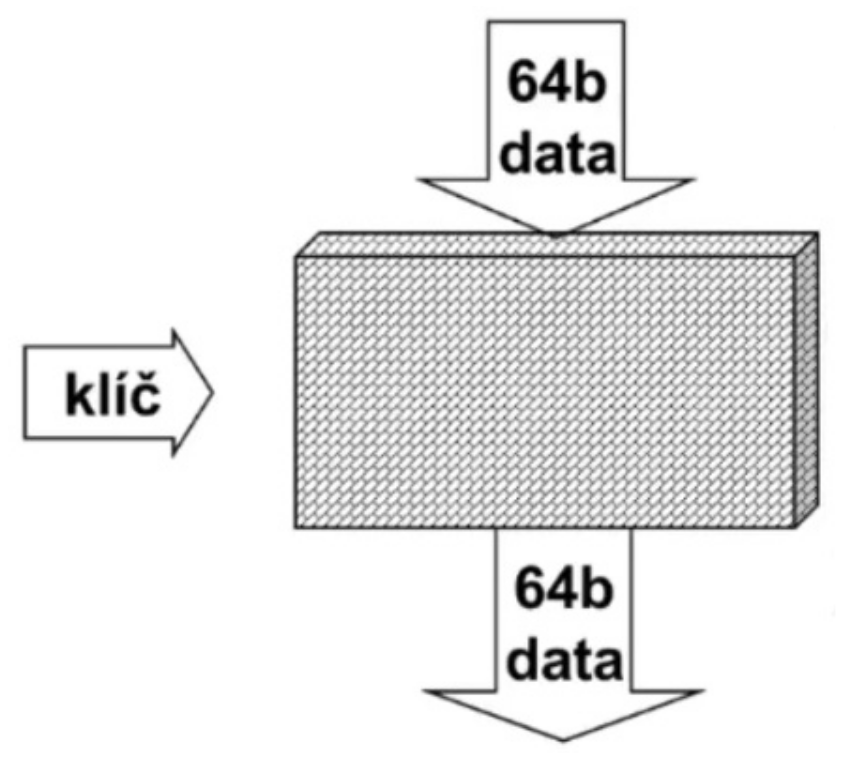
\includegraphics[width=0.35\linewidth]{50/symmetric_cryptography_blocks.png}
    \caption{Princip blokových šifer.}
\end{figure}

\subsection*{Feistelova šifra}

Feistelova šifra (Feistelův princip) je koncept šifrování, který konkrétní algoritmy využívají. Jedná se o substituční-permutační síť. Vstupní blok je rozdělen na dvě poloviny $L$ a $R$, výpočet výstupu pak vypadá následovně.

\begin{equation}
    L_i = R_{i-1}
\end{equation}

\begin{equation}
    R_i = L_{i-1} \oplus F(R_{i-1}, K_i)
\end{equation}

\paragraph*{Funkce F} $F$ je funkce, na kterou Feistelova šifra neklade žádné požadavky. Jednotlivé algoritmy, využívající Festelovu šifru, funkci samy definují. Požadavky na funkci $F$, aby algoritmus byl bezpečný: \begin{itemize}
    \item skrytí vlastností zprávy;
    \item skrytí vlastností zprávy.
\end{itemize}

\paragraph*{Subklíč} K je tzv. subklíč, který je generován typicky nějakým pseudonáhodným generátorem na základě inicializačního klíče (hlavní).

\paragraph*{Dešifrování} Dešifrování se provádí stejným způsobem, pouze pořadí subklíčů je opačné.

\begin{figure}[H]
    \centering
    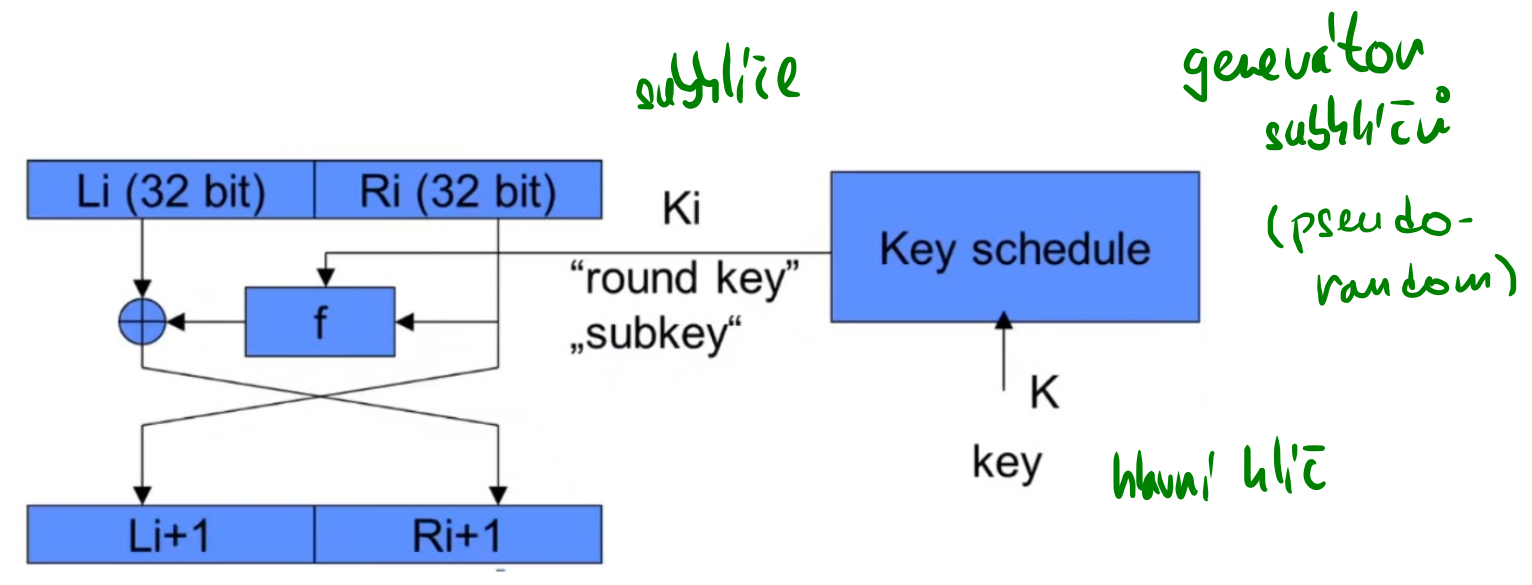
\includegraphics[width=1\linewidth]{50/feistel.png}
    \caption{Jeden krok opakování (Feistelův krok) vizuálně.}
\end{figure}

\begin{figure}[H]
    \centering
    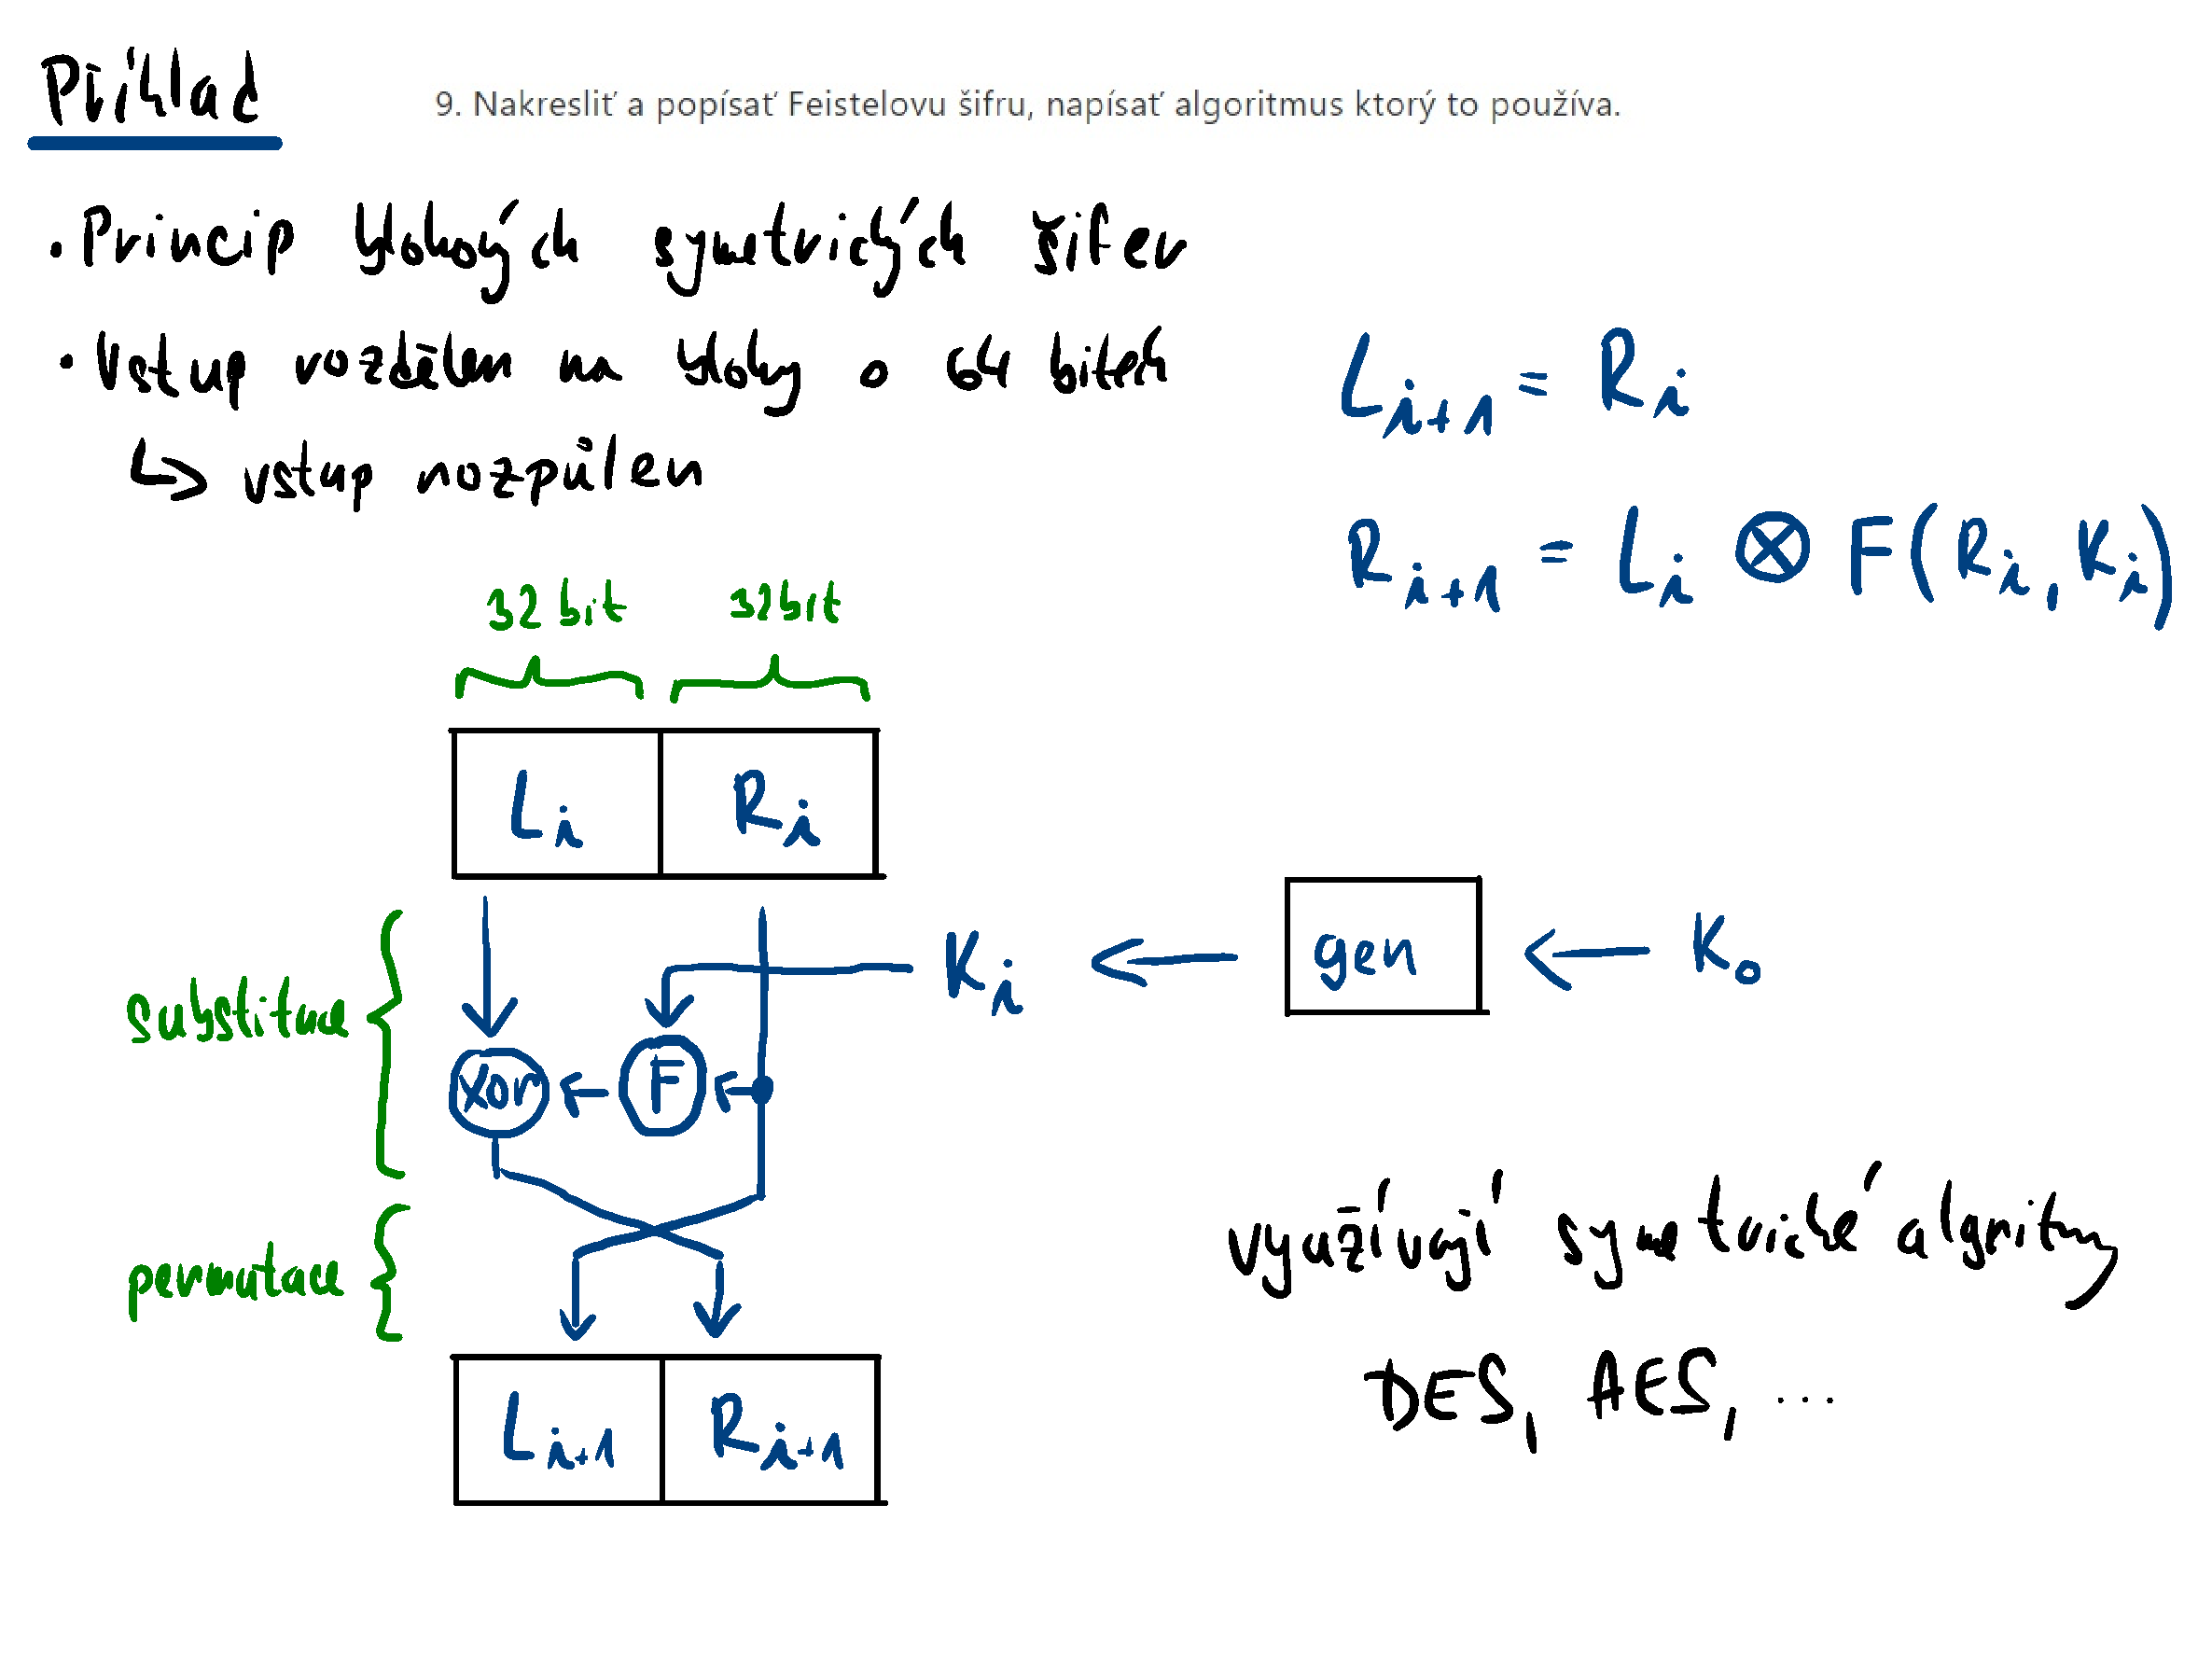
\includegraphics[width=1\linewidth]{50/feistel_example.pdf}
    \caption{Feistelova šifra -- příklad a rekapitulace.}
\end{figure}

\subsection*{Data Encryption Standard (DES)}

DES byl první algoritmus s veřejnou specifikací (\textit{security by design}). Využívá princip Feistelovy šifry -- 16 kol. Dodatečně přidává na začátek a konec permutaci navíc. Klíč je dlouhý 64b (resp. 56 významových bitů a 8 paritních).

\paragraph*{Slabiny} \begin{itemize}
    \item 56 bitový klíč je příliš krátky a je možný útok silou.
    \item Rozdílná velikost bloku a klíče (zvláštnost).
    \item Existence slabých a poloslabých klíčů.
    \item Není jasné proč zrovna 16 iterací a zda je to dostatečné.
\end{itemize}

\begin{figure}[H]
    \centering
    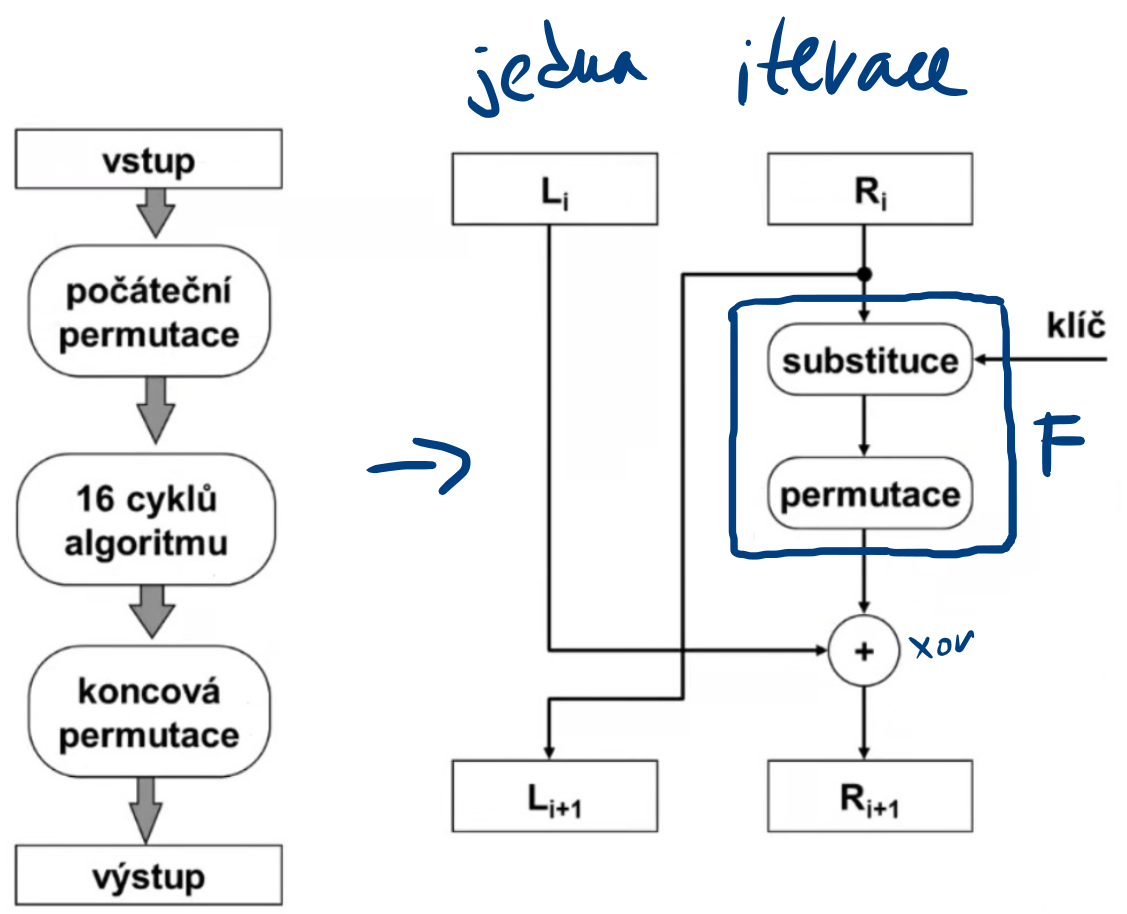
\includegraphics[width=0.75\linewidth]{50/des_schema.png}
    \caption{DES -- Schéma fungování algoritmu.}
\end{figure}

\begin{figure}[H]
    \centering
    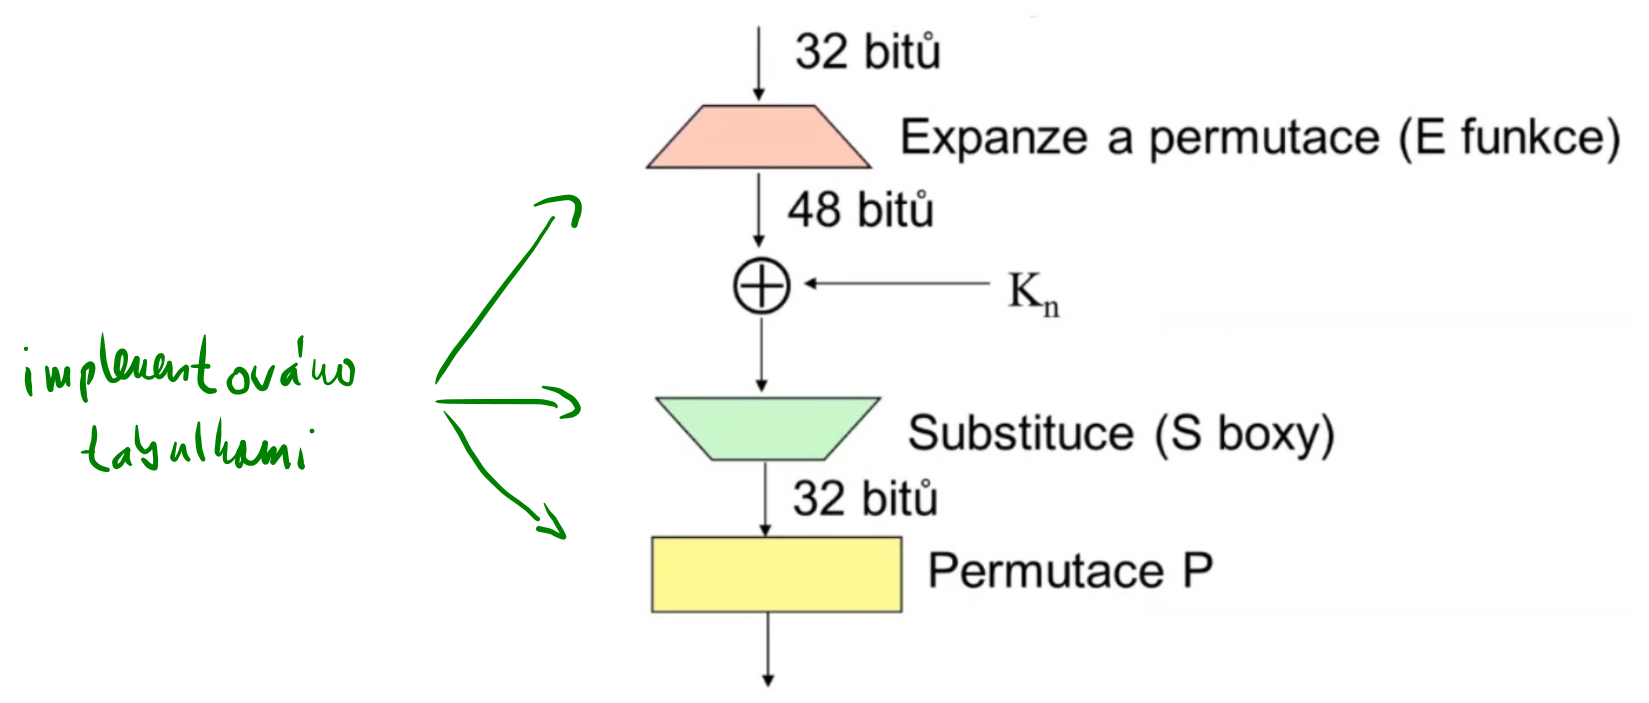
\includegraphics[width=1\linewidth]{50/des_f.png}
    \caption{DES -- funkce F.}
\end{figure}

\begin{figure}[H]
    \centering
    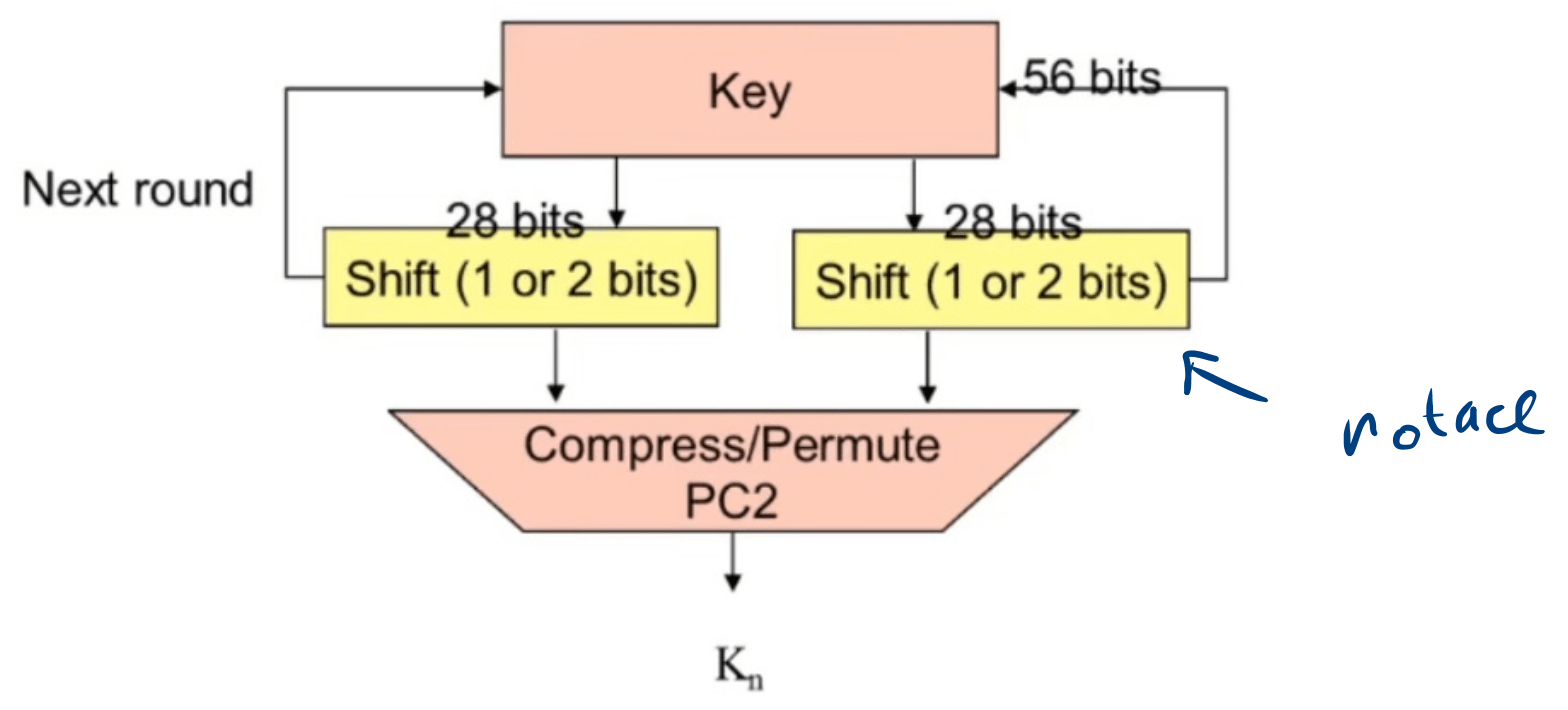
\includegraphics[width=1\linewidth]{50/des_keys.png}
    \caption{DES -- generování subklíčů.}
\end{figure}

\begin{figure}[H]
    \centering
    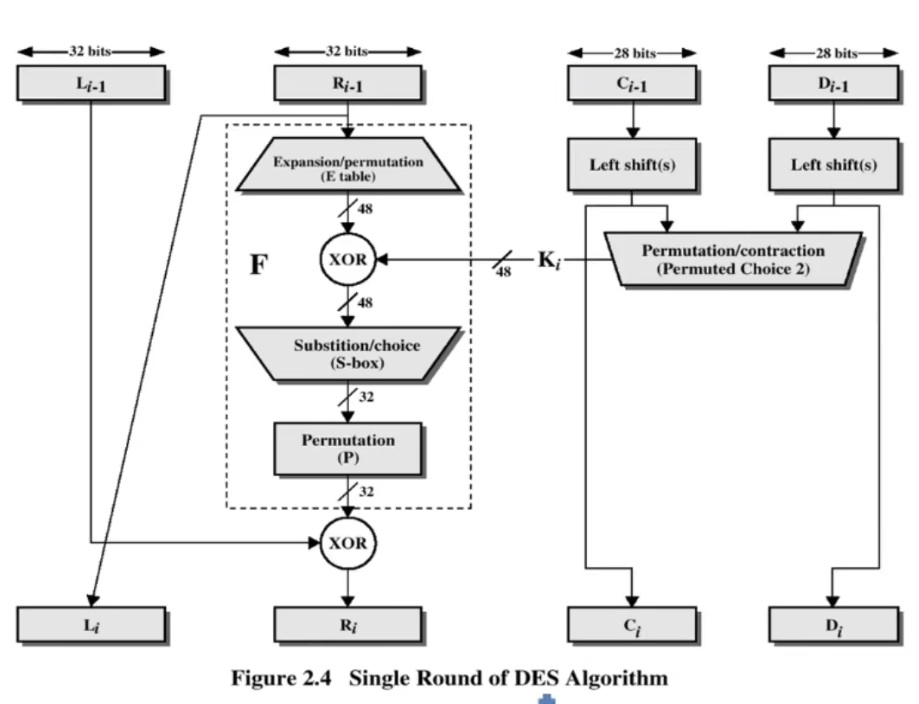
\includegraphics[width=1\linewidth]{50/des_single_round.png}
    \caption{DES -- jedno kolo algoritmu. \textit{Left shift} je ve skutečnosti bitová rotace.}
\end{figure}

\begin{figure}[H]
    \centering
    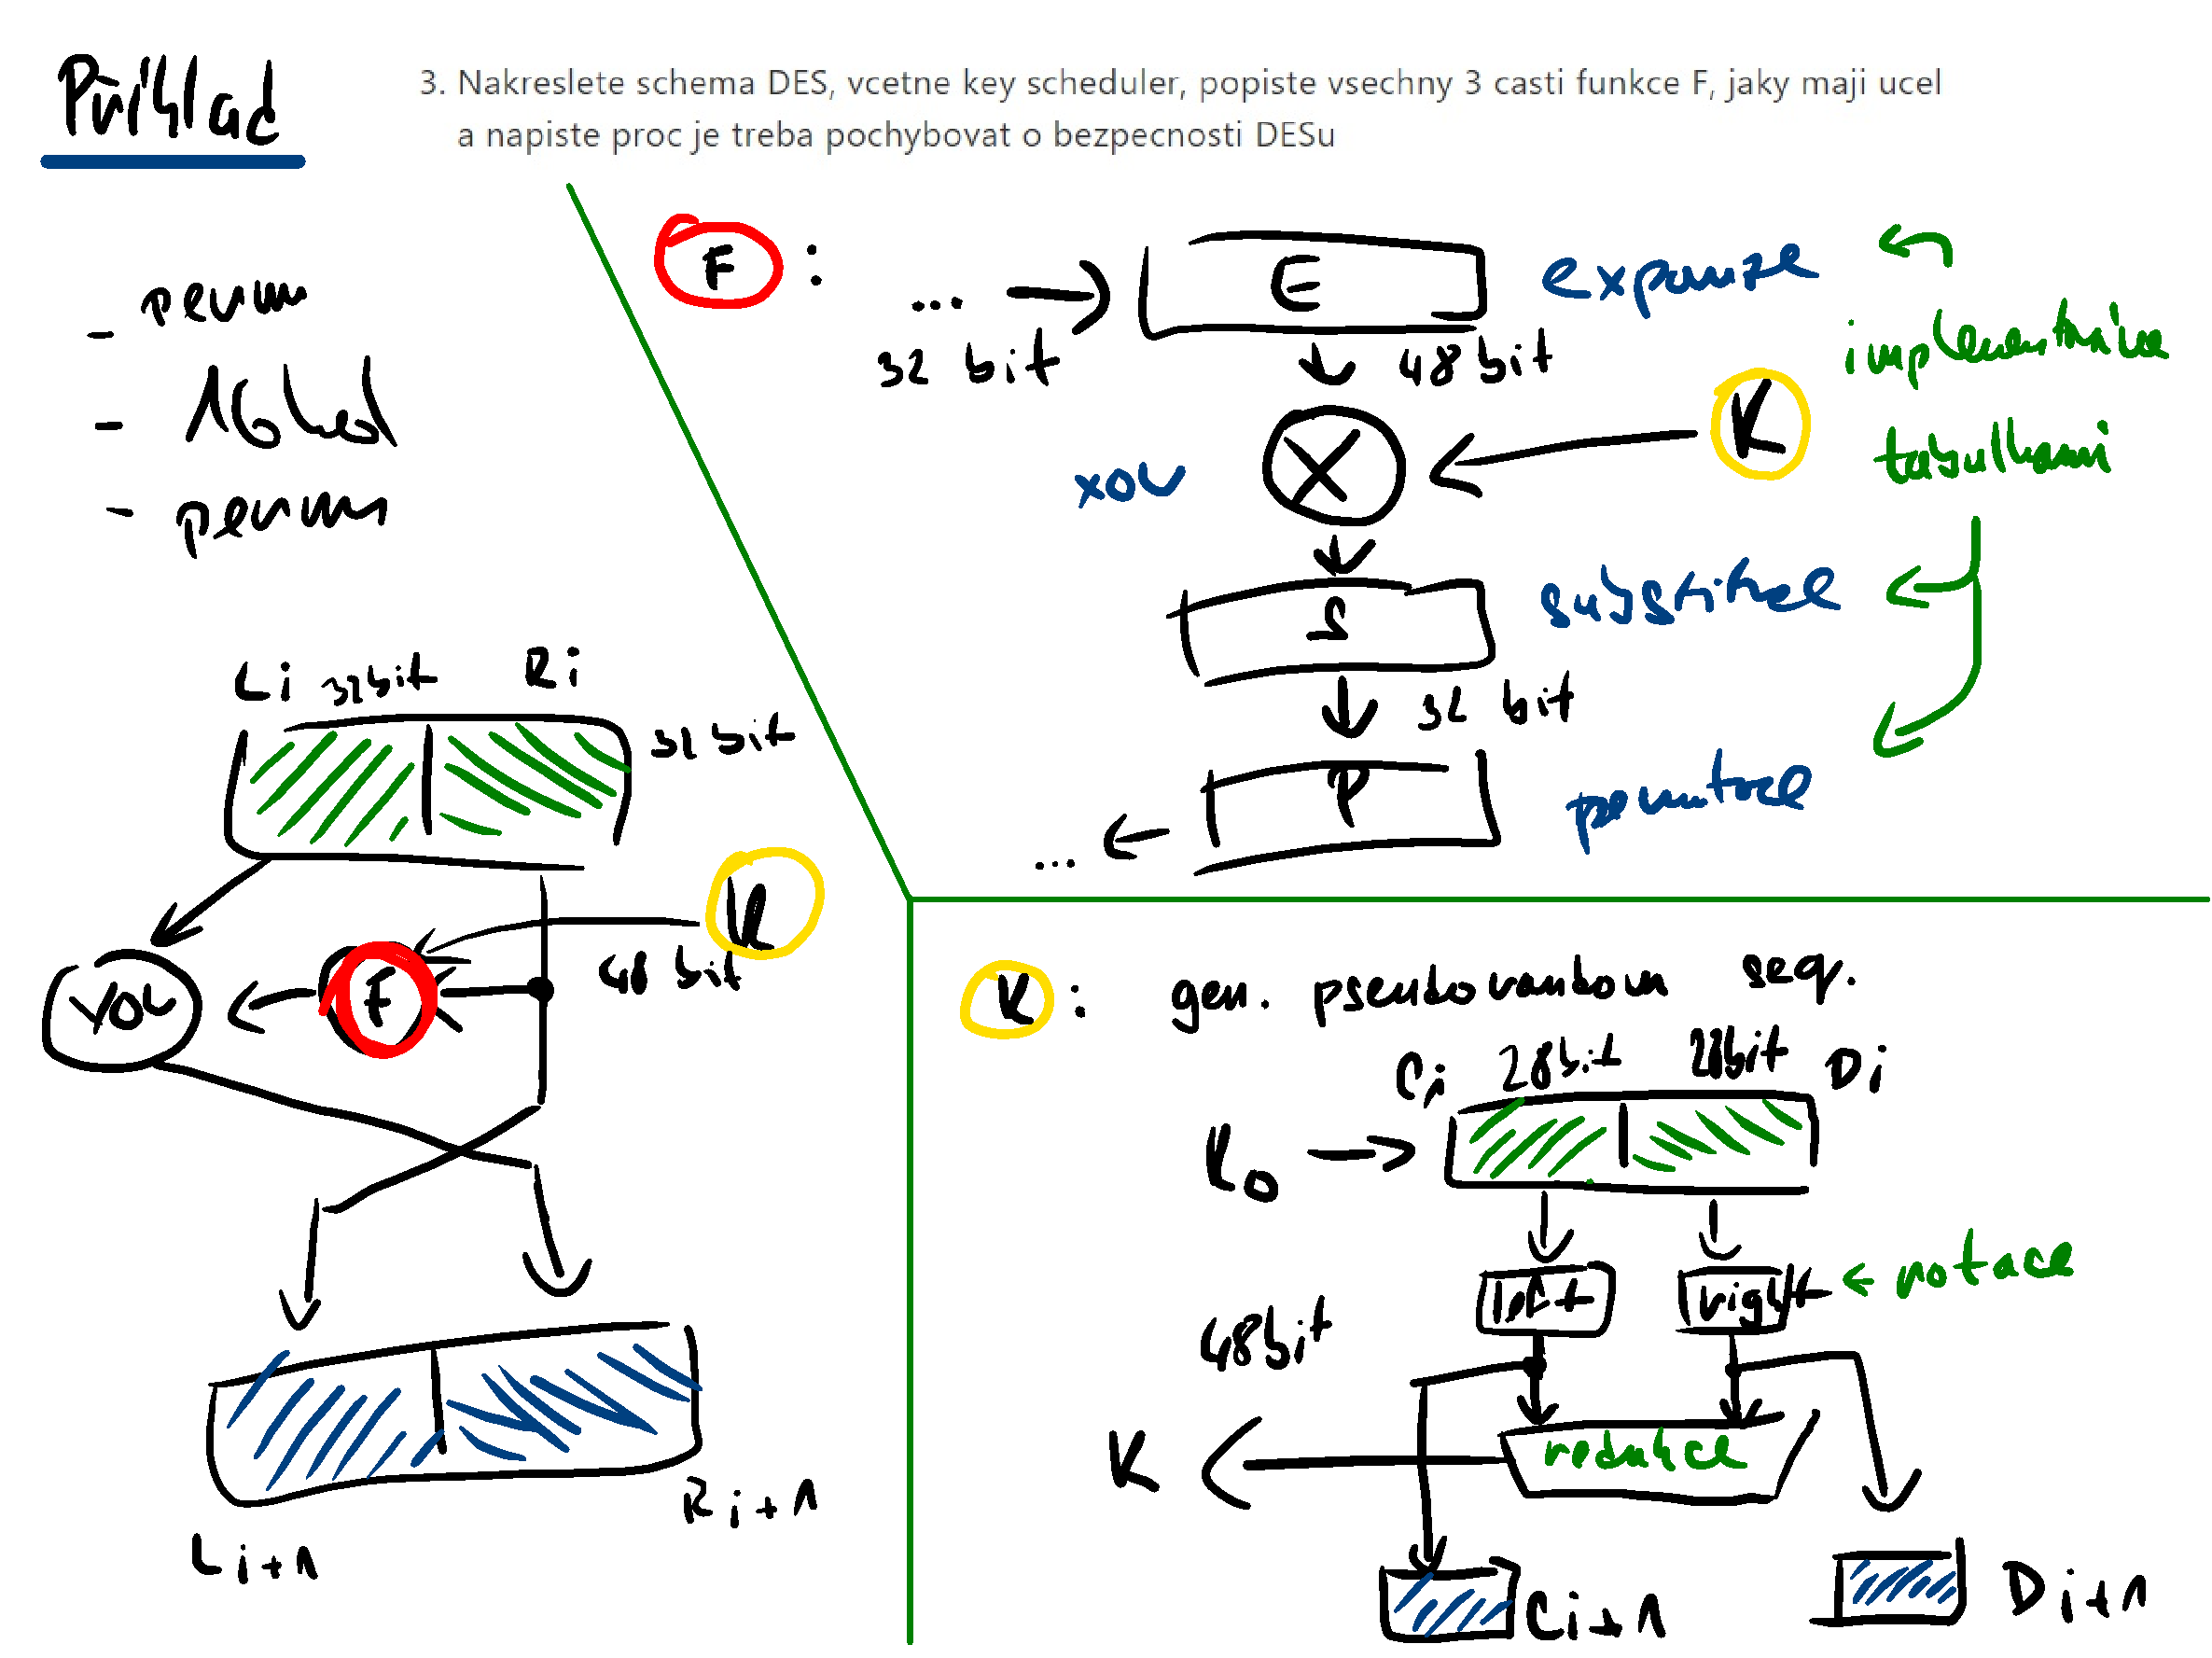
\includegraphics[width=1\linewidth]{50/des_example.pdf}
    \caption{DES -- příklad a rekapitulace.}
\end{figure}

%%%%%%%%%%%%%%%%%%%%%%%%%%%%%%%%%%%%%%%%%%%%%%%%%%%%%%%%%%%%%%%%%%%%%%%%%%%%%%%%

\section{Provozní režimy činnosti blokových šifer}

Slabinou blokových šifer, pomocí které může kryptoanalýza šifru prolomit, je opakované použití stejné transformace (stejného klíče) na všechny bloky. Proto je nutné použít nějaký druh provozního režimu blokové šifry. Ten vnese do šifrování další vstup, který způsobí, že zašifrovaná data vypadají jako náhodná sekvence. Tento doplňující náhodný vstup (inicializační vektor), může způsobit, že bloková šifra se chová jako proudová.

\subsection*{Electronic Code Book (ECB)}

\todo{todo}

\subsection*{Cipher Block Chaining (CBC)}

\todo{todo}

\subsection*{Cipher Feedback (CFB)}

\todo{todo}

\subsection*{Output Feedback (OFB)}

\todo{todo}

\subsection*{Counter (CTR)}

\todo{todo}

%%%%%%%%%%%%%%%%%%%%%%%%%%%%%%%%%%%%%%%%%%%%%%%%%%%%%%%%%%%%%%%%%%%%%%%%%%%%%%%%

\section{Proudové šifry}

\todo{todo}

\subsection*{Synchronní proudové šifry}

\todo{todo}

\subsection*{Samosynchronizující proudové šifry}

\todo{todo}

\subsection*{Generátory PRNG}

\todo{todo}
